\section{Evaluation}
\label{sec:evaluation}

  \subsection{Exhaustive search vs \atl orthogonal search}
  \label{sec:exhaustiveVSorthogonal}
  \begin{figure*}[tbhp]
    \centering
    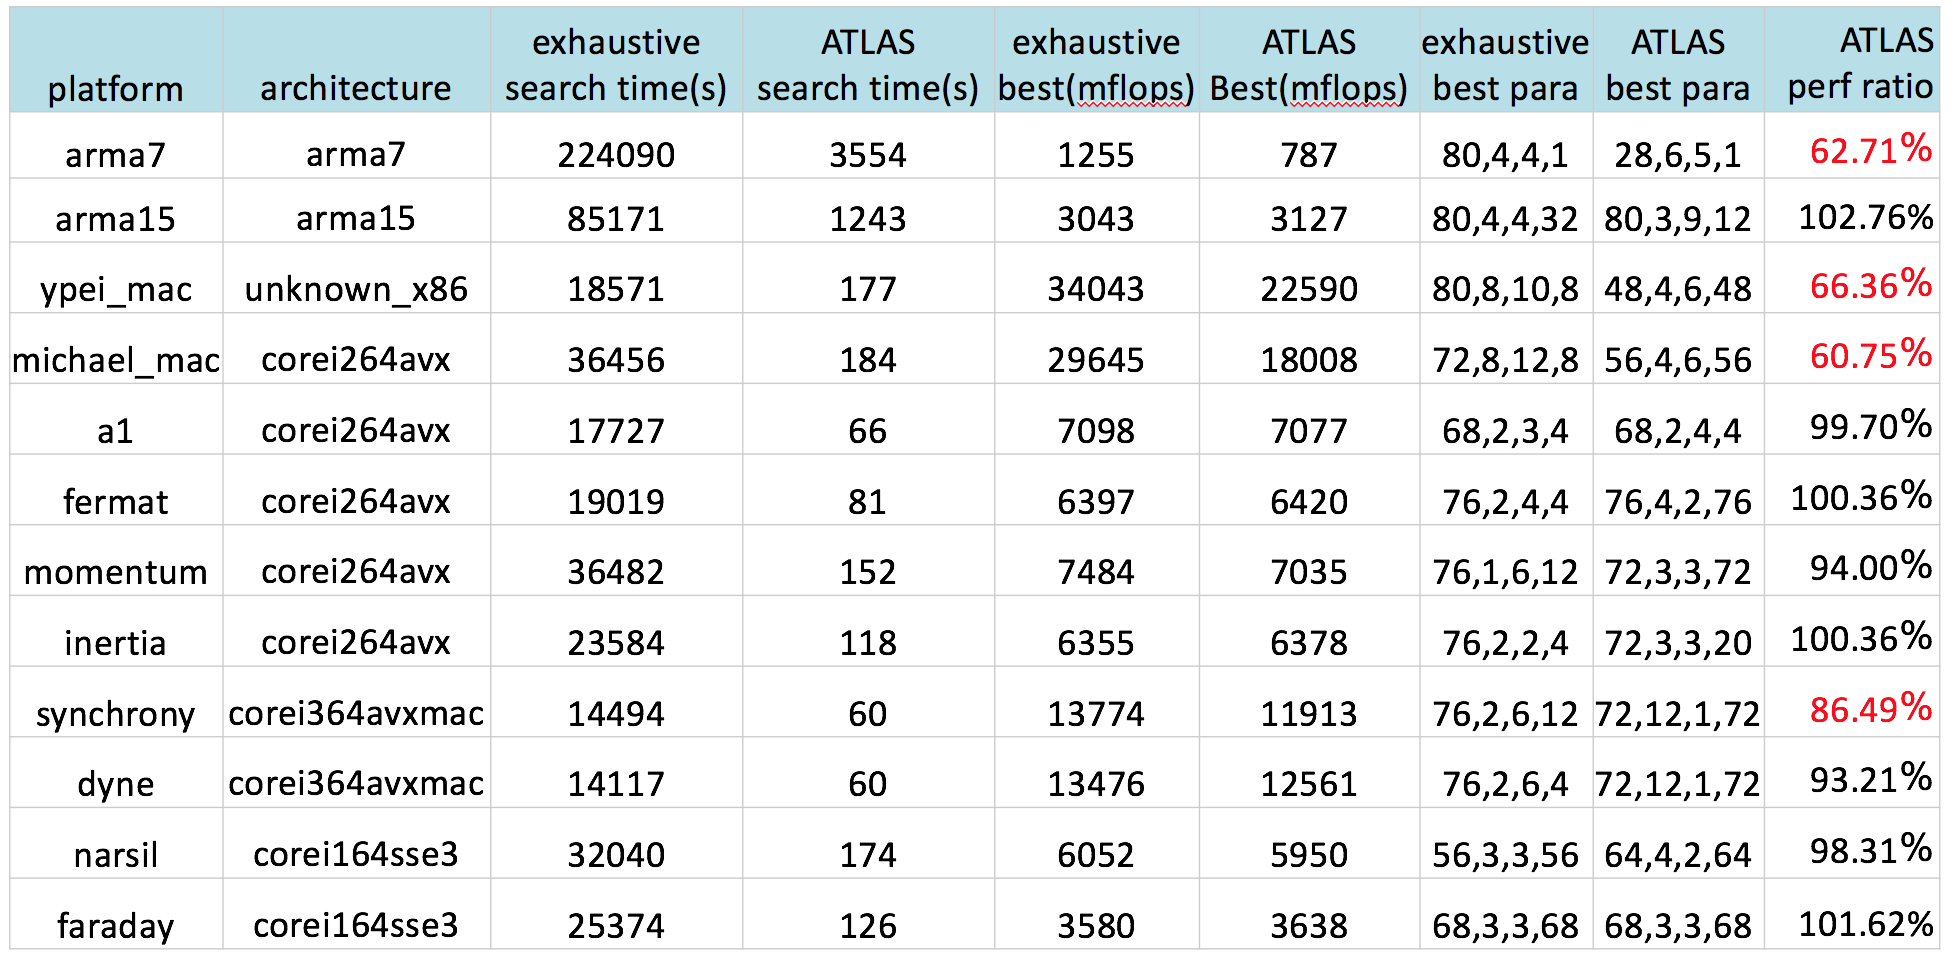
\includegraphics[width=0.9\textwidth]{images/exhaustiveVsorthogonal.png}
    \caption{Searching time comparison between exhaustive search and \atl orthogonal search}
    \label{fig:exhaustiveVsorthogonal}
  \end{figure*}
  In this section, we compare the result of \atl orthogonal search with the best of exhaustive
  search. The search time, generated code performance, and selected parameters are listed in Figure
  \ref{fig:exhaustiveVsorthogonal}.\par
  Except for the two ARM processors, it takes around one to three minutes for ATLAS orthogonal search
  to generate its best code. Considering that we only search for single precision, real number general
  matrix multiplication, we haven't run double precision, complex number or some other benchmarks
  like transpose matrix kernel, matrix vector kernel, big matrix kernel, rank-1 matrix kernel etc, installing
  ATLAS may take hours to finish. The orthogonal search is still too slow to end user.\par
  Column \textit{exhaustive best} and \textit{ATLAS best} list the MFLOPS performance of generated code from
  both search strategy. The ratio of ATLAS over exhaustive is in the last column. On 8 platforms,
  ATLAS is able to generate code with >90\% of best performance. Three platforms has only around 60\% of
  best performance. The two parameter columns list the selected parameters in the order of $(NB, MU, NU, KU)$.\par
  Note for the two MAC platform that, the two middle parameters (MU, NU) are so large that it exceeds
  the register requirement of \[ MU*NU + MU + NU + LS < NR \]. Thus ATLAS orthogonal search is not able
  to find it. Currently we do not have a clear explanation to this. One guess is that, the CORE i7 processors
  have more physical registers than ISA architecture register. The ISA is only able to use or identify 32 registers.
  However due to register renaming, it can make use of more than 32 registers and the extra registers are not visible
  to softwares.\par

  \subsection{GEMM performance model}
  \label{sec:GEMMperf}
  This section discuss whether it is easy to build a model of \gem performance
  given platform information and a knob setting. Intuitively, we evaluate
  whether the \gem performance is predictable. In Fig.\ref{fig:inertia_perf},
  we shows the performance prediction accuracy on platform inertia using a model
  trained by M5 on the other 11 platforms. Each point represent one knob
  setting. This figure shows the comparison between the normalized actual
  performance and the predicted performance. There are two views to evaluate
  this figure. The first view is to see the distance between the points to the
  $y=x$ line. The distance evaluates how accurate the model is.

  Another point of
  view is to focus on the few highest data points, which are the points in the
  red oval in Fig.\ref{fig:inertia_perf}. These points represent the highest
  predicted performance, which will be selected as the candidate knob settings
  in \atl evaluation. The corresponding x axis value is the actual performance
  number for this knob setting. Intuitively, the lefter the point is, the
  better the prediction is, we want high prediction to indicate high actual
  performance. Note that only the knob settings with high performance are
  interested, so the prediction accuracy for low points doesn't matter much in
  this case as soon as high prediction point are left enough.

  Inertia is doing well in both of the views, while platforms like arma7 is not
  because it's really hard to use data collected from 10 Intel processors and 1
  ARM processor to predict another ARM processor's performance, as shown in
  Fig.\ref{fig:arm_perf}. The overall performance prediction, shown in
  Fig.\ref{fig:overall_perf}, is generated by randomly selecting 80\% and 20 \%
  of the data set formed by 12 platforms as training data and testing data
  respectively. It shows the overall difficulty of modeling \gem performance
  is not hard.

  \begin{figure}[bhp]
    \centering
    \begin{subfigure}[b]{1.0\linewidth}
      \centering
      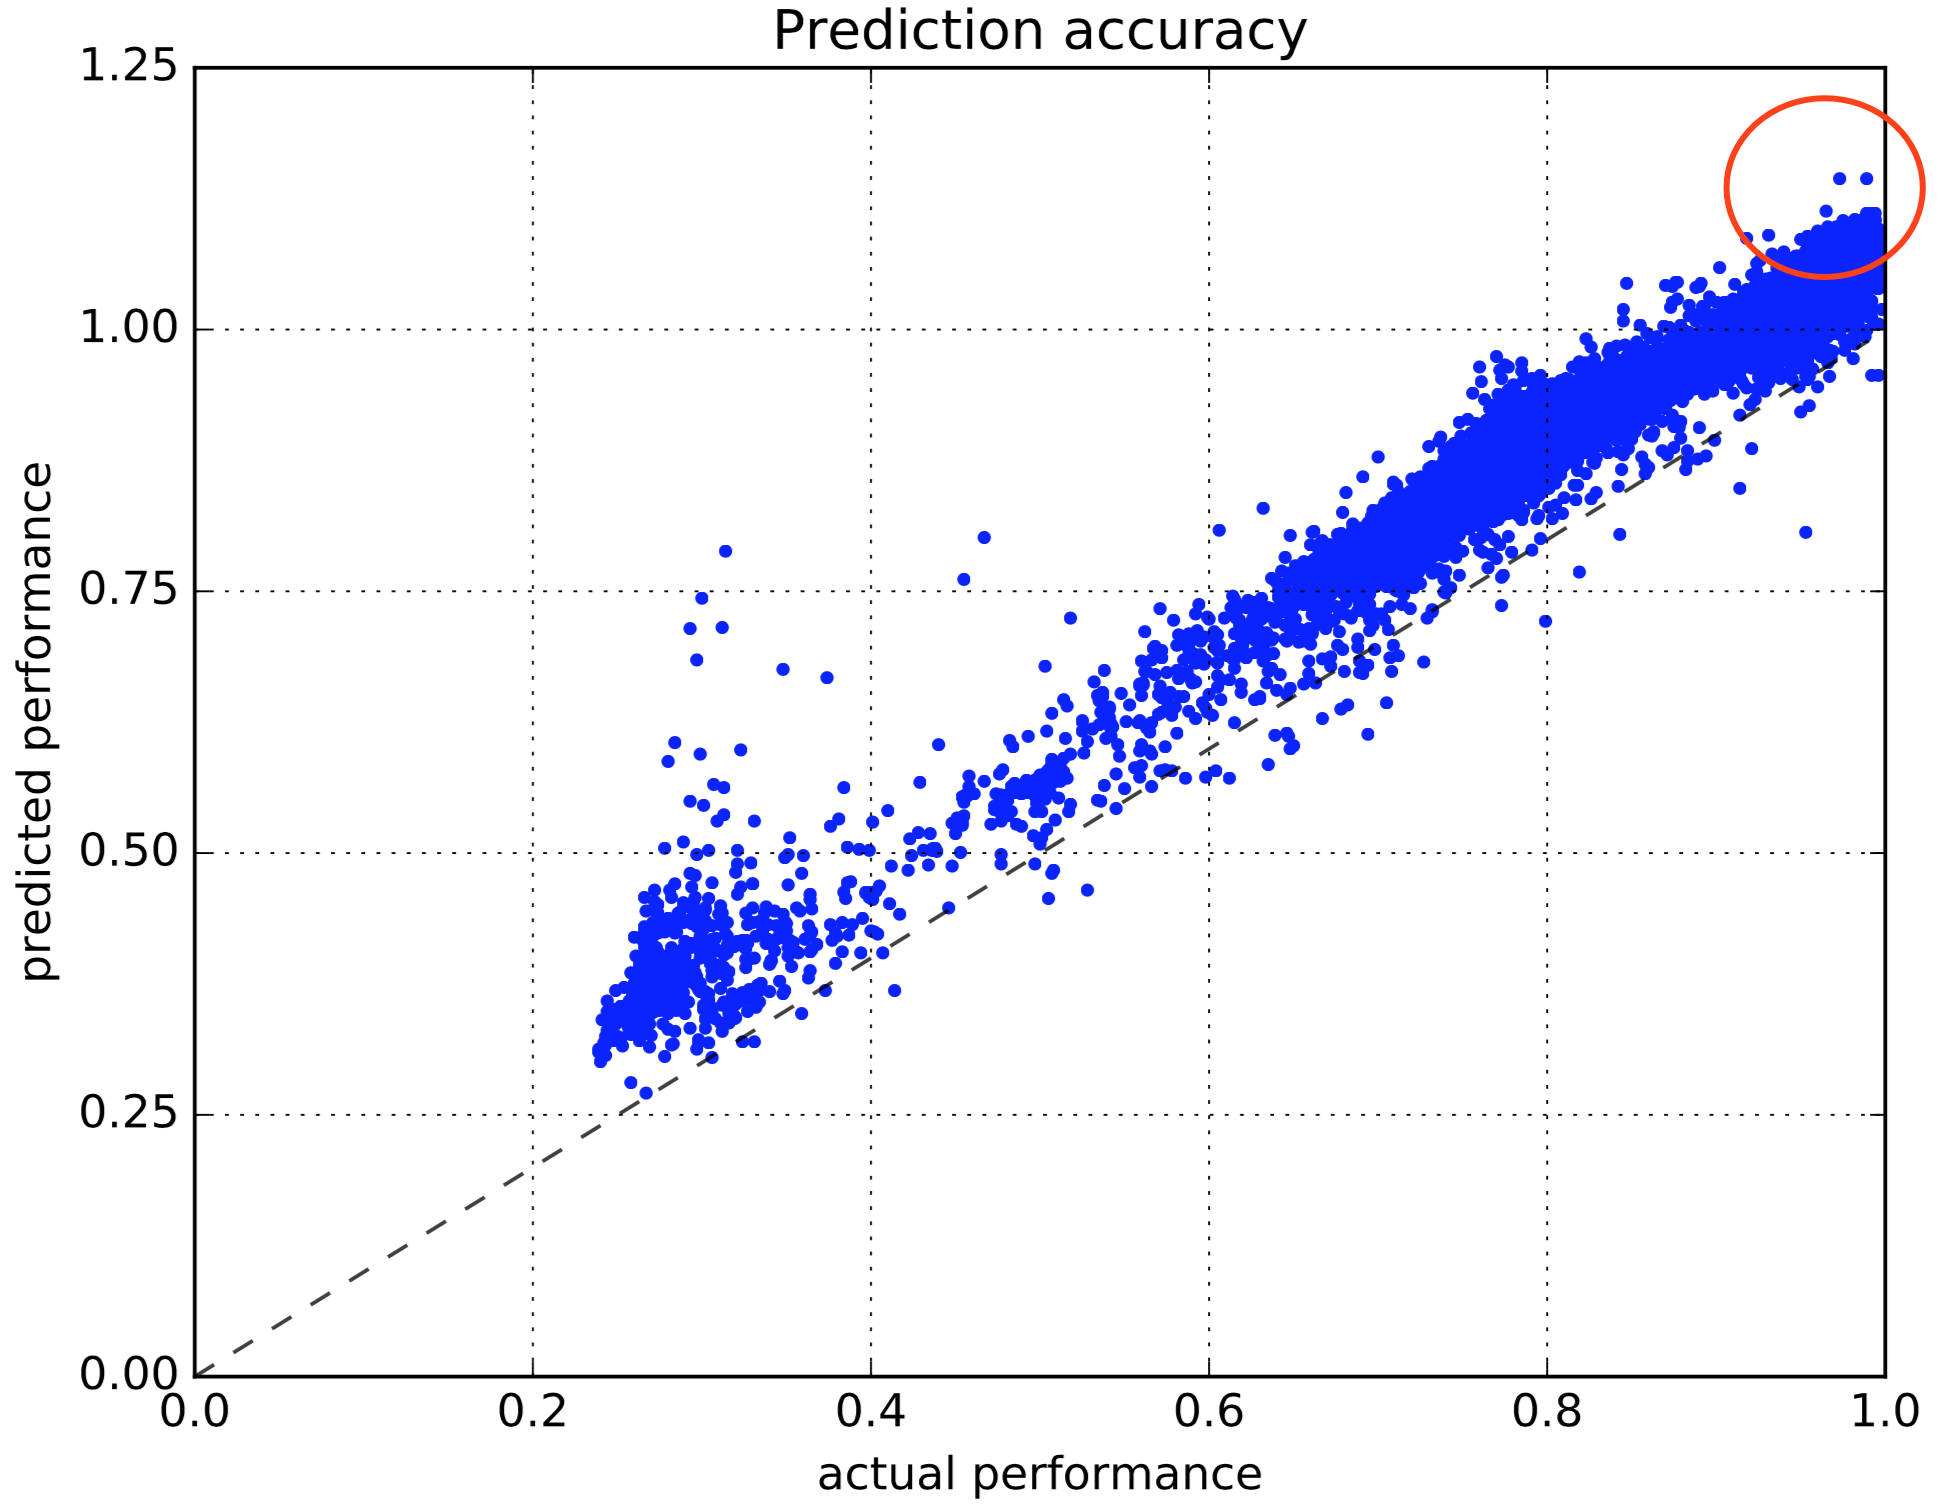
\includegraphics[width=0.8\textwidth]{images/inertia_perf.png}
      \caption{Inertia performance prediction}
      \label{fig:inertia_perf}
    \end{subfigure}
    \begin{subfigure}[b]{1.0\linewidth}
      \centering
      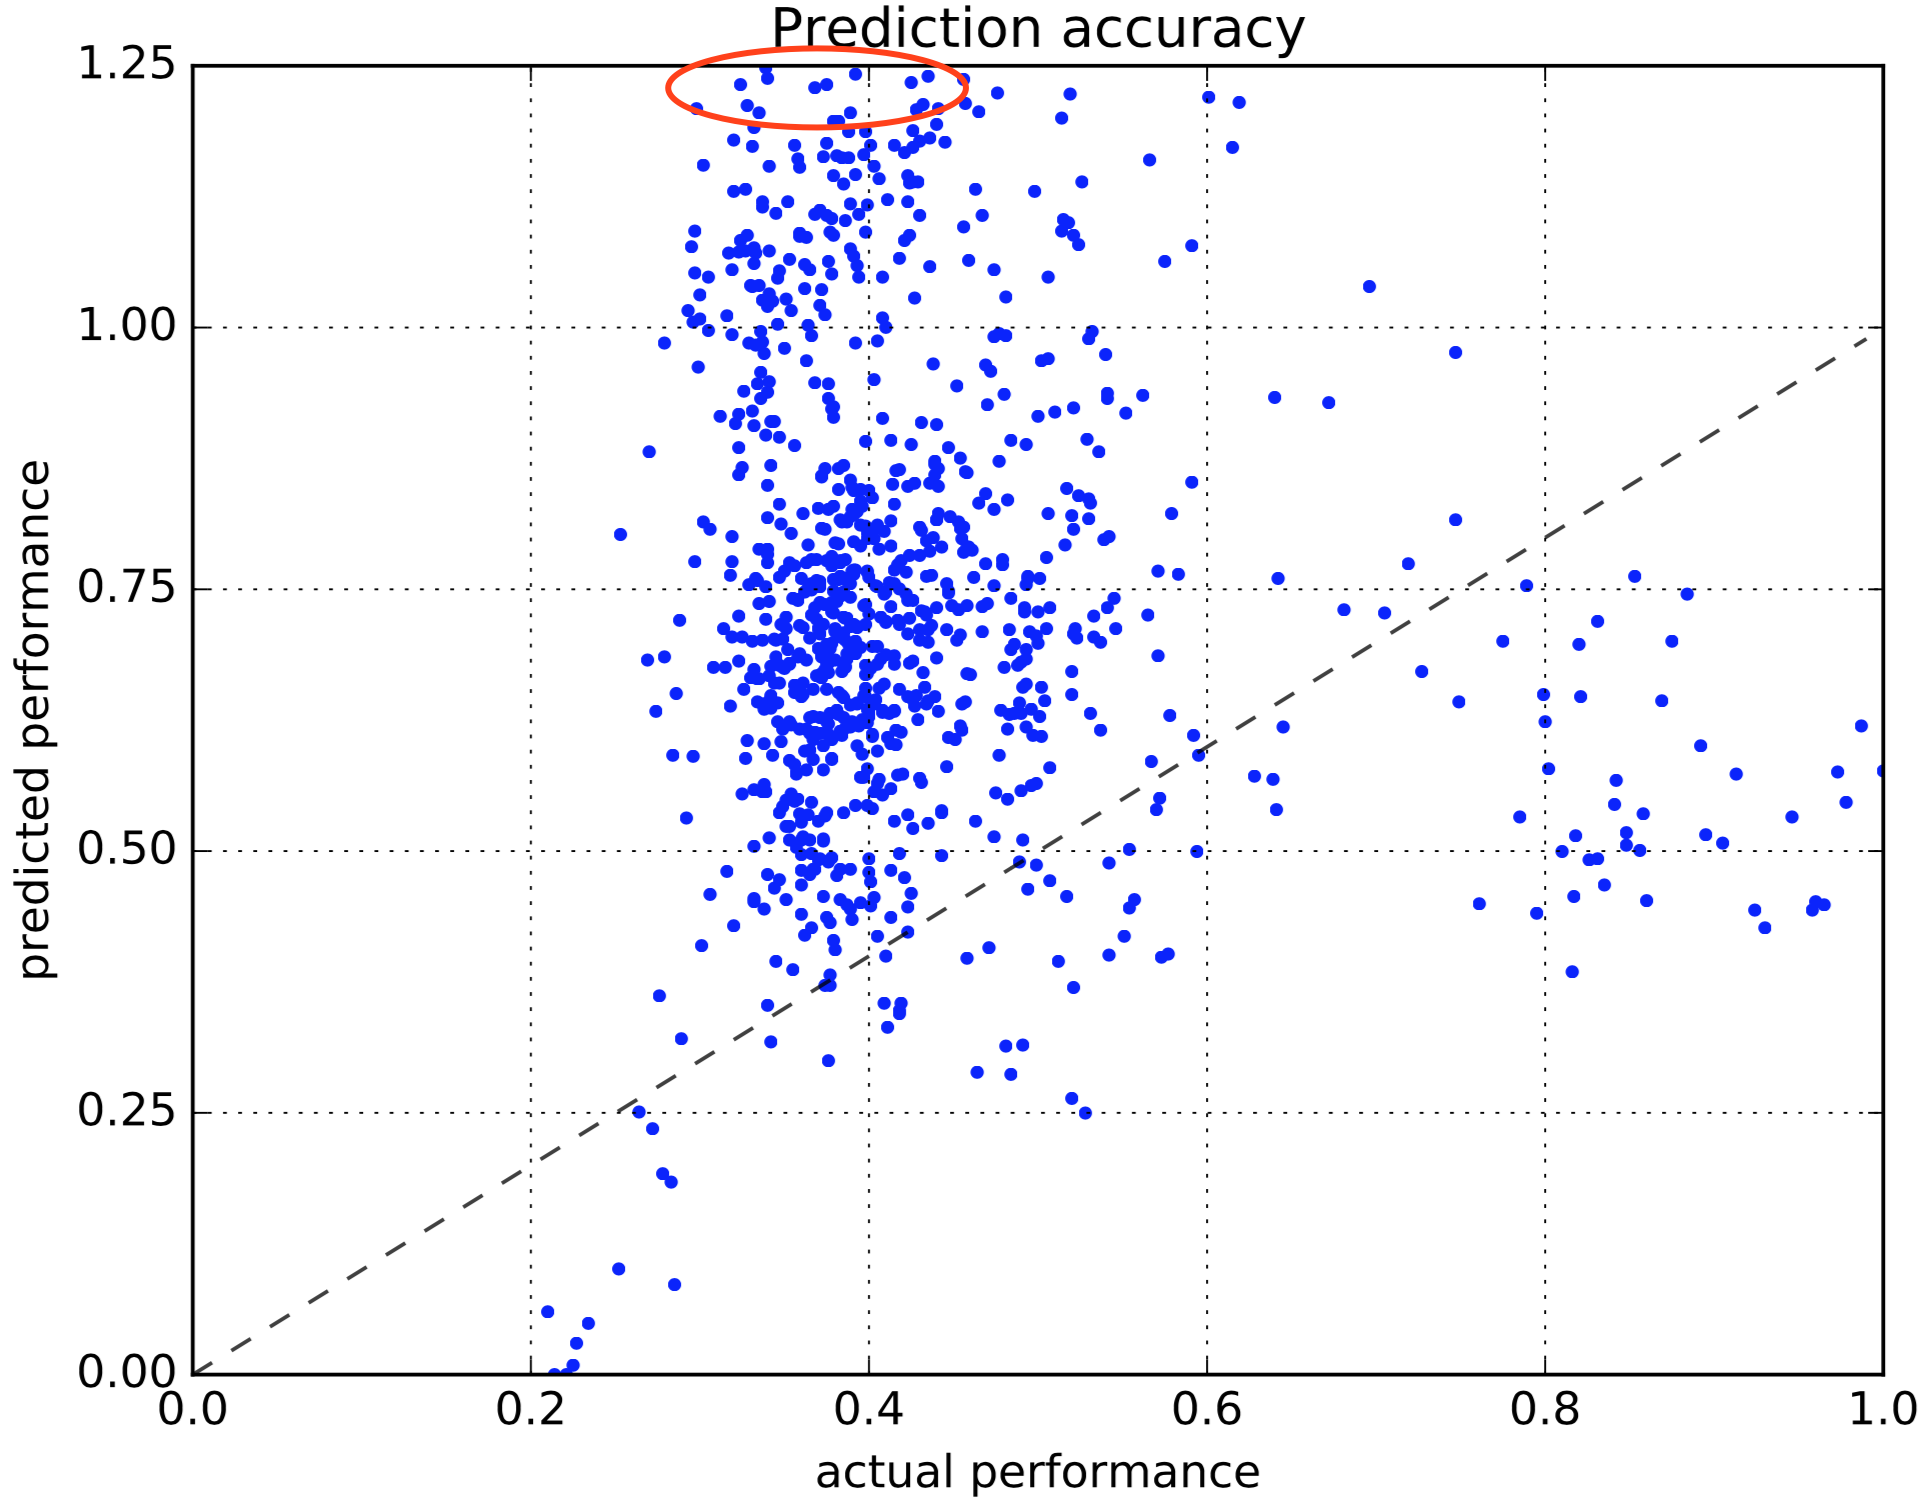
\includegraphics[width=0.8\textwidth]{images/arm_perf.png}
      \caption{Arma7 performance prediction}
      \label{fig:arm_perf}
    \end{subfigure}
    \begin{subfigure}[b]{1.0\linewidth}
      \centering
      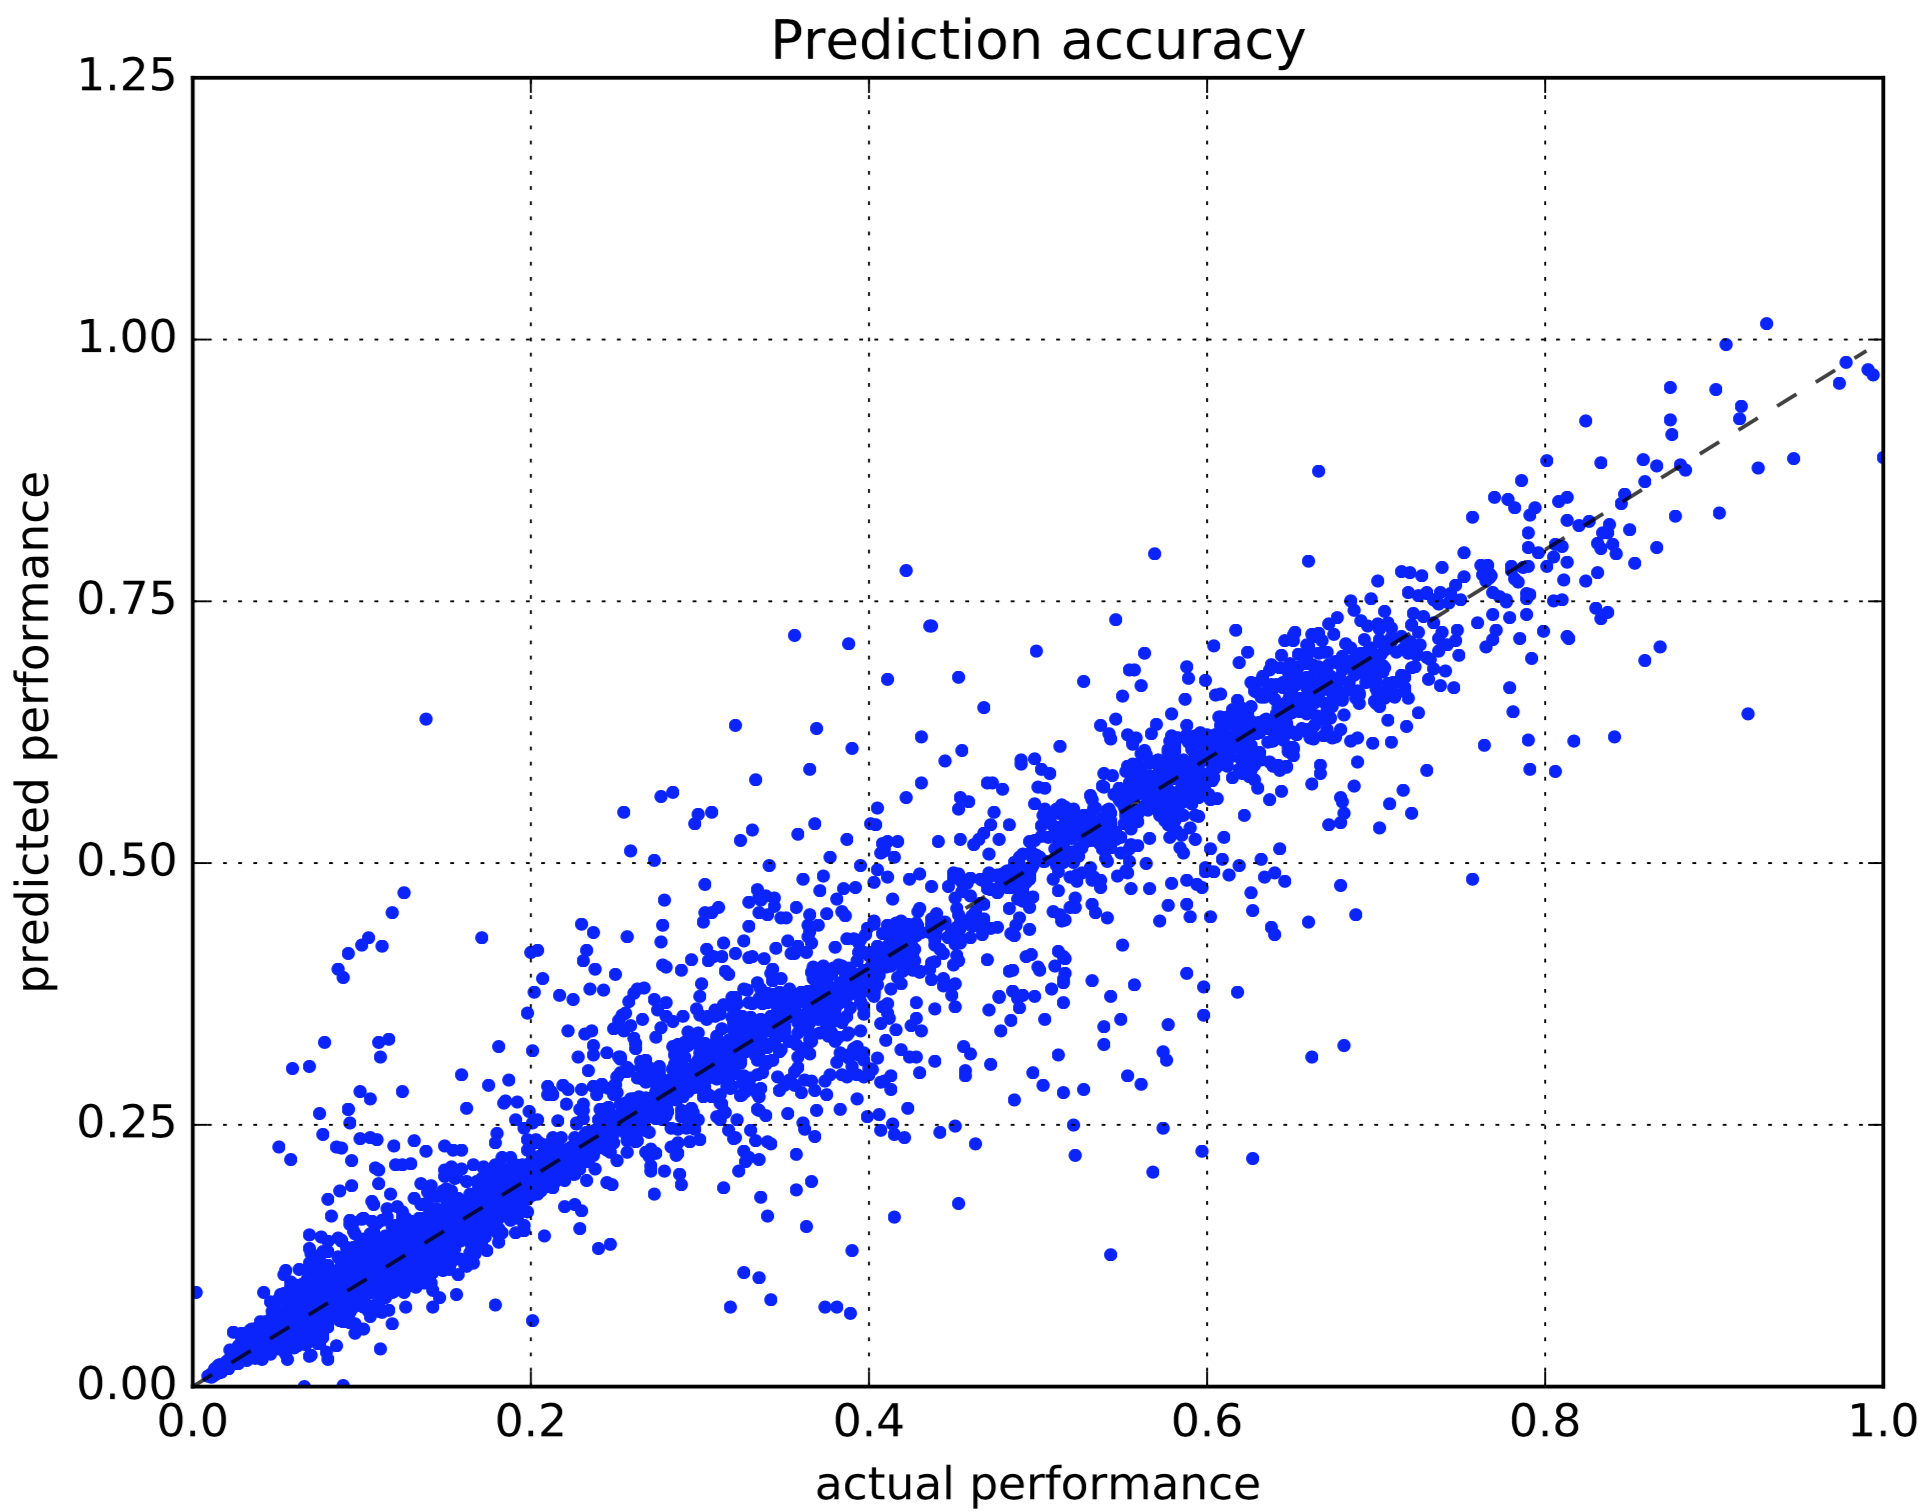
\includegraphics[width=0.8\textwidth]{images/overall_model.png}
      \caption{Overall performance prediction}
      \label{fig:overall_perf}
    \end{subfigure}
  \end{figure}


  
  \subsection{Capri-based ATLAS searching time}
  \label{sec:capri_atlas_searching}
  In this section we compare one of our evaluation metric: searching time. An overview of the result is listed in
  Figure \ref{fig:search_time}. The \textit{ATLAS search time} column is the same as in Figure \ref{fig:exhaustiveVsorthogonal}.
  \textit{Capri search time} shows the time Capri takes to purely generate top candidates without running them. 
  \textit{Capri runtime per candidates} is the average time of each candidate running on the actual platform.
  Therefore, total Capri-based ATLAS search time which is the sum of \textit{Capri search time} and actual platform time of the candidates,
  highly depends on how many candidates that the user wants. The last two columns show the speedup over ATLAS when users pick
  10 or 5 candidates. On average, Capri-based search outperforms ATLAS orthogonal search by \textbf{10.88X} on 10 candidates and \textbf{17.97X} on 
  5 candidates. On the two ARM platforms, Capri-based search can even reach more than 200X speedup.
  


  \begin{figure*}[tbhp]
    \centering
    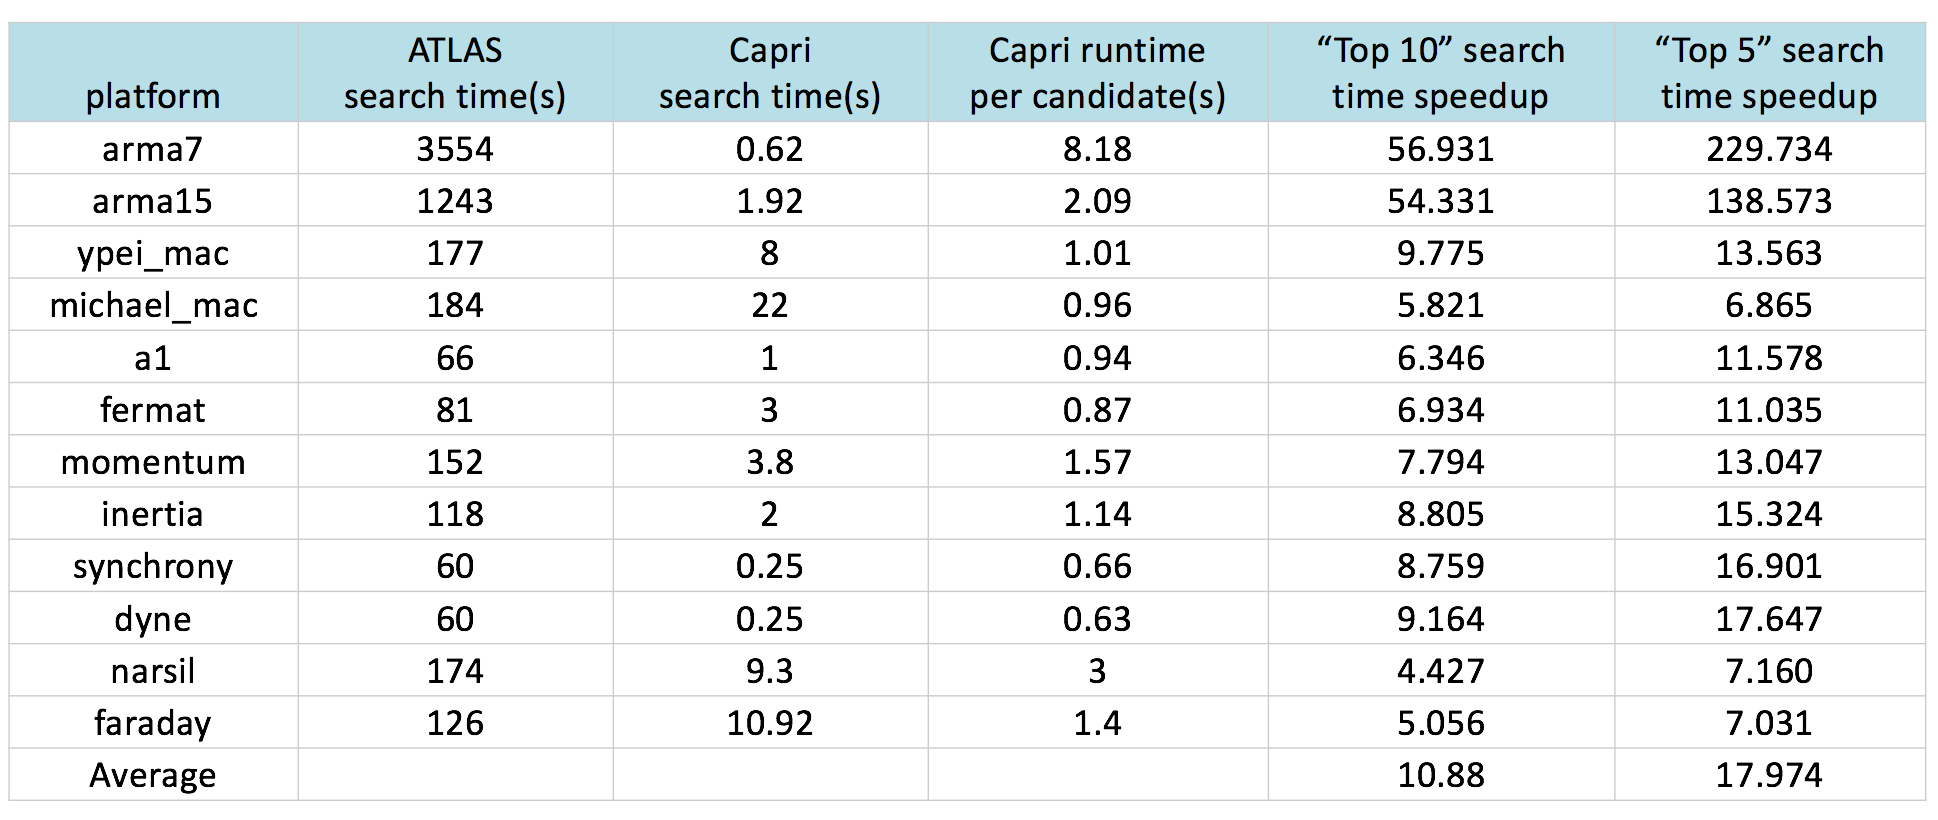
\includegraphics[width=0.9\textwidth]{images/timespeedup.png}
    \caption{Capri-based ATLAS searching time speedup}
    \label{fig:search_time}
  \end{figure*}

  \subsection{Capri-based ATLAS performance}
  \label{sec:capri_atlas_performance}

  \begin{figure*}[tbhp]
    \centering
    \begin{subfigure}[b]{1.0\linewidth}
      \centering
      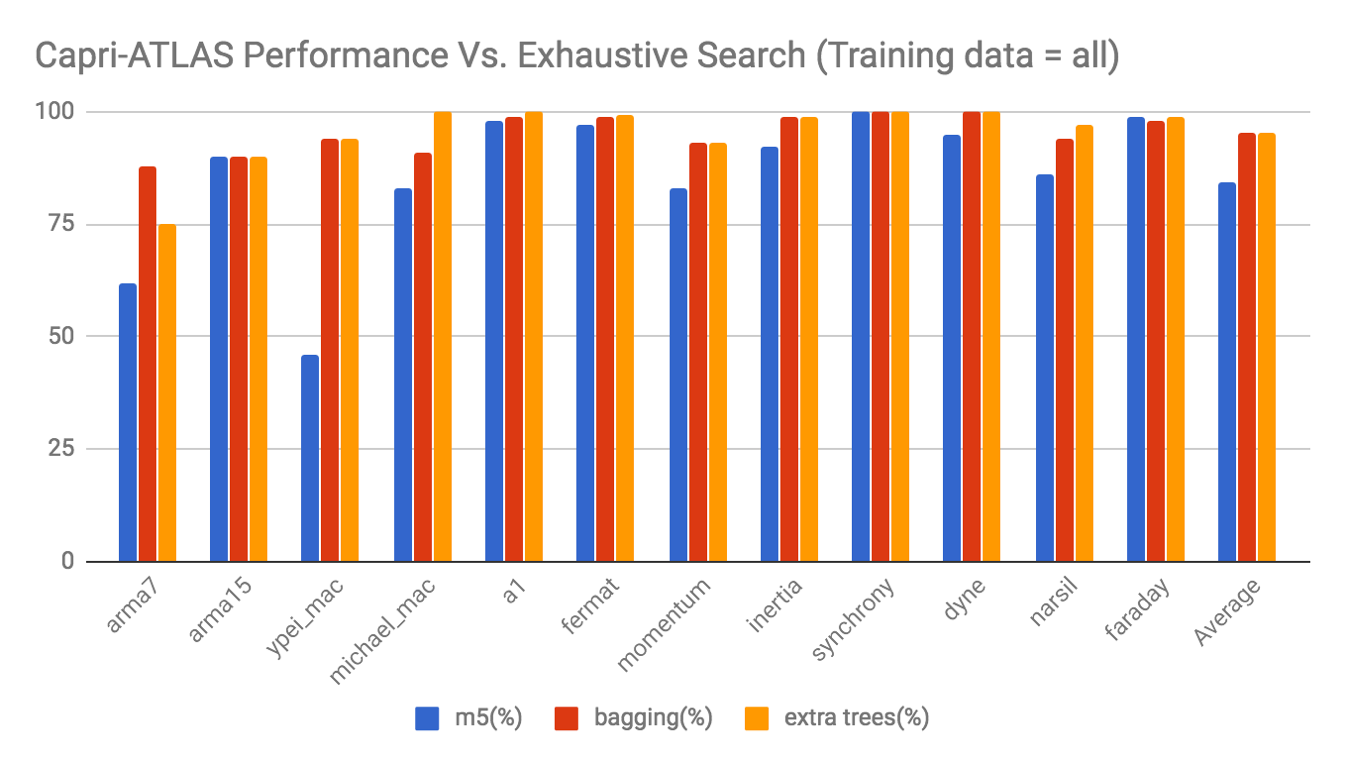
\includegraphics[width=0.85\textwidth]{images/all_perf.png}
      \caption{ }
      \label{fig:all_perf}
    \end{subfigure}
    \begin{subfigure}[b]{1.0\linewidth}
      \centering
      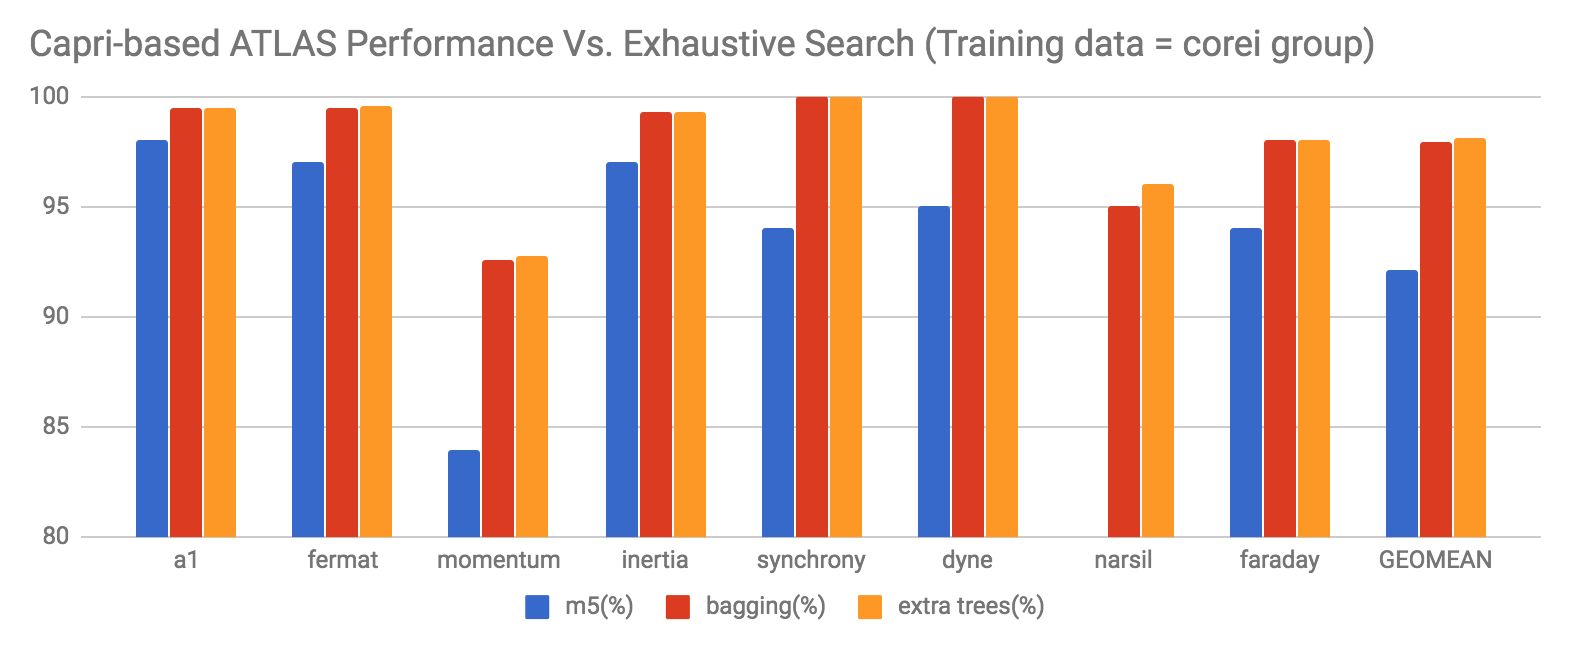
\includegraphics[width=0.85\textwidth]{images/corei_perf.png}
      \caption{ }
      \label{fig:corei_perf}
    \end{subfigure}
    \begin{subfigure}[b]{1.0\linewidth}
      \centering
      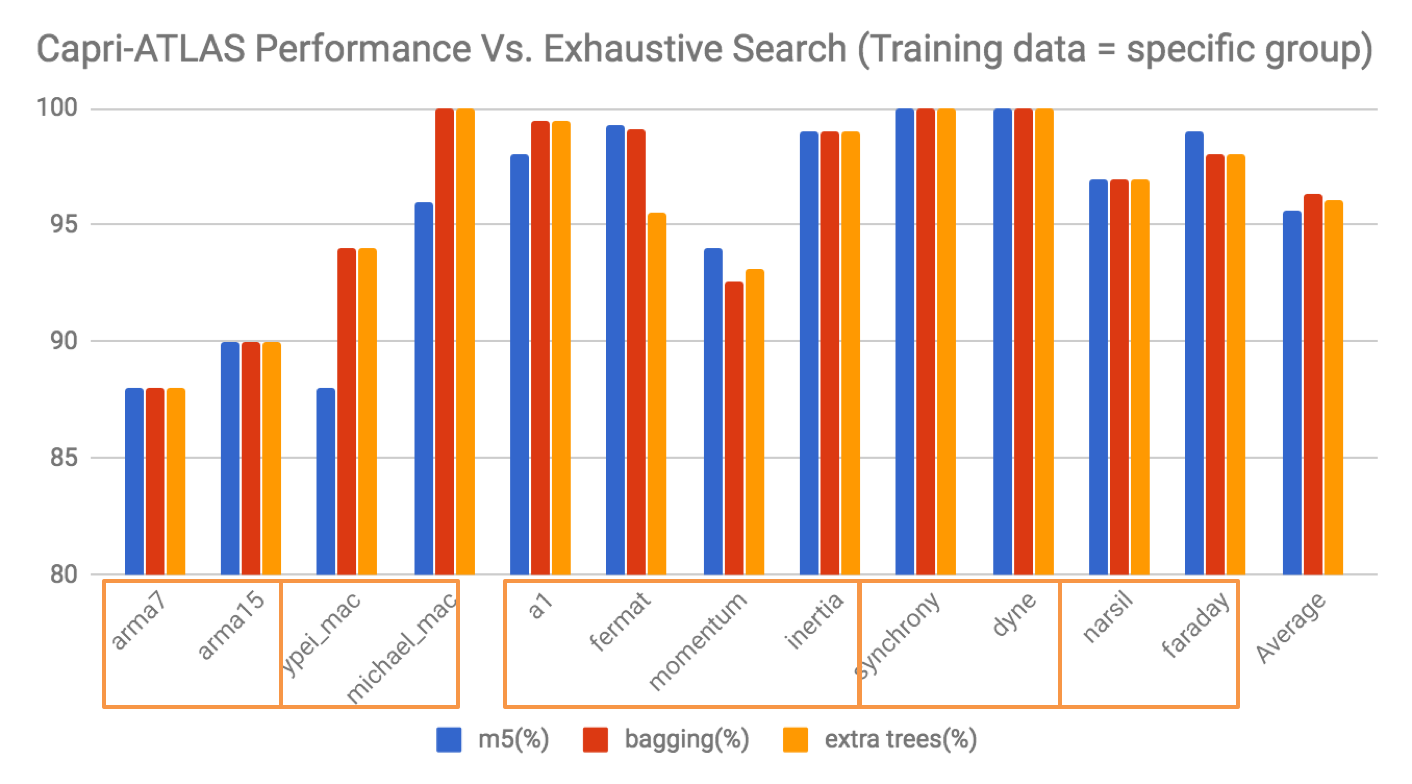
\includegraphics[width=0.85\textwidth]{images/specific_perf.png}
      \caption{ }
      \label{fig:specific_perf}
    \end{subfigure}
  \caption{Capri-based \atl Performance using different training sets}
  \end{figure*}

  \subsection{Parameter sensitivity}
  \label{sec:parametersensitivity}
  \begin{figure*}[tbhp]
    \centering
    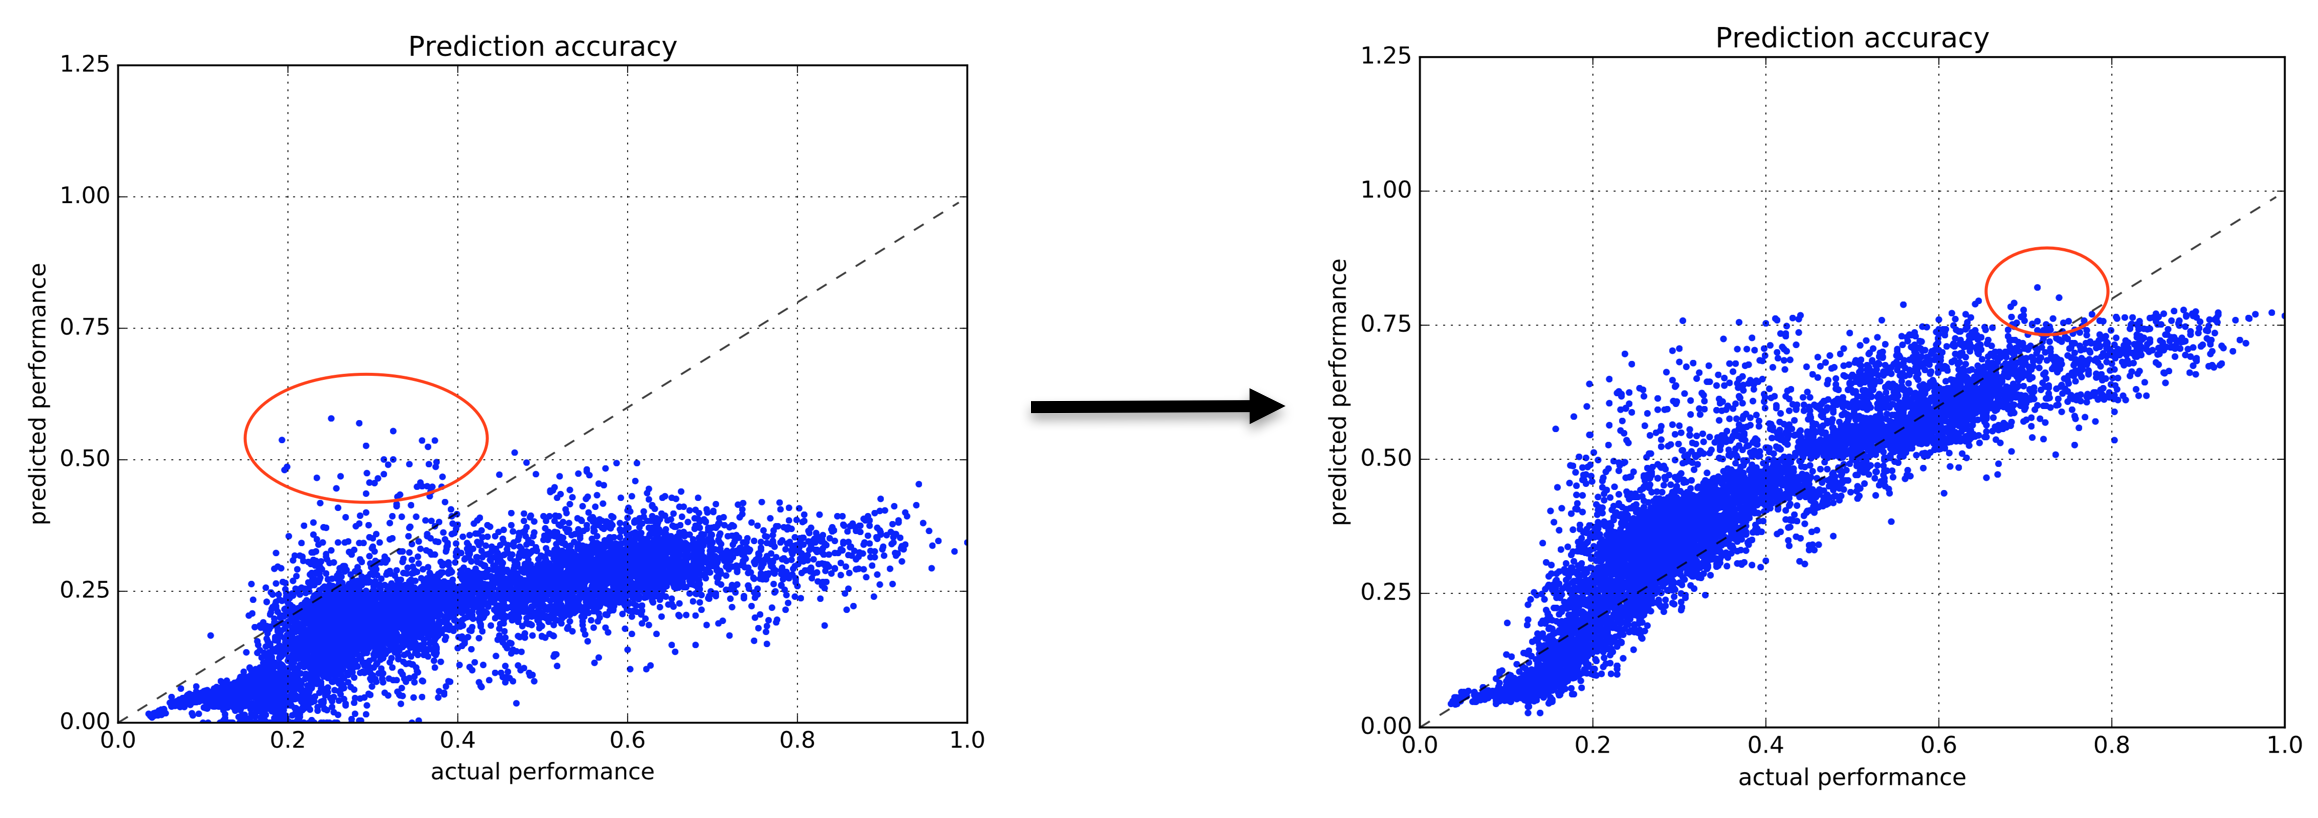
\includegraphics[width=0.9\textwidth]{images/ypei_perf_change.png}
    \caption{Performance improves when a better training set is selected}
    \label{fig:ypei_perf_change}
  \end{figure*}

    \subsubsection{Training set}
    \label{sec:training_set}

    \subsubsection{Top M constraint}
    \label{sec:top_m}
